\section{Principle}
\label{sec:principle}
%
%
Our proposed lens combines the modification of several parameters of a typical DVR rendering of volume data, as follows. Consider the typical DVR algorithm: Given a scalar volume $V \subset \mathbf{R}^3 \rightarrow \mathbf{R}$, each pixel $\mathbf{x} \in I$ in the DVR image $I \subset \mathbf{R}^2$ thereof corresponds to the compositing of sampled data along a ray starting passing through $V$ and ending at $\mathbf{x}$. In classical DVR (\autoref{f:fisheye}-a), such rays are defined by the eye position $\mathbf{e}$ and a viewing direction vector $\mathbf{d}$ pointing from $\mathbf{e}$ to $\mathbf{x}$. Consider next a 2D focus point $\mathbf{f} \in I$ (the \emph{lens center}) and a lens radius $R > 0$. In our proposal, we modify all rays traveling through the 2D disk $D = \{\mathbf{x} \in I | \| \mathbf{x} - \mathbf{f} \| \leq R\}$, or \emph{focus area}, in order to de-occlude, magnify, and emphasize a target object. Our new ray behavior can be divided into four steps: (1) Provide an unobstructed view of the occluded object. This moves closer to the target while avoiding the obstacles by pushing them aside. (2) Set a wide field-of-view (fisheye) to better see the target. (3) Smoothly vary several DVR parameters between the focus $D$ and the \emph{context} $I \setminus D$ to better emphasize objects in focus while maintaining context. (4) Interactively modify various lens parameters in real time so as to better explore the object in focus. These steps are detailed next.

\subsection{Creating an unobstructed view}
\label{sec:gathering}
%
The key situation our lens addresses is as follows: Given a volume $V$, users produce a DVR thereof, using whatever suitable TFs and other parameters their application considers. When examining $V$ from various viewpoints, (at least) one viewpoint $(\mathbf{e},\mathbf{d})$ is found from which some intriguing structure is \emph{partially} visible in $I$. Users next want to quickly and easily unravel this structure. For this, our first step proceeds as follows: We first \emph{gather} all rays passing through from the lens pixels (focus area $D$) to follow the lens' axis vector $\mathbf{f} - \mathbf{e}$. As explained above, at the location $\mathbf{f}$ of the lens center, we do see an interesting partially occluded structure. Hence, by definition, the gathered rays pass \emph{through} occluders to hit this structure, otherwise we would not see it. In detail, we control the gathering by setting the ray direction passing through $\mathbf{x} \in D$ to $\mathbf{r}(\mathbf{x}) = (1-\alpha)(\mathbf{f} - \mathbf{e}) + \alpha (\mathbf{x} - \mathbf{e})$, with $\alpha \in [0,1]$. When $\alpha=0$, the rays all follow the lens axis, thus, are most gathered to squeeze through obstacles. When $\alpha=1$, rays follow their original classical DVR path (not squeezed).
\subsection{Setting a wide field of view}
%
Once the rays pass obstacles (by suitable setting of the viewpoint $(\mathbf{e},\mathbf{f})$ and ray gathering, as described in Sec.~\ref{sec:gathering}, we next want to \emph{scatter}rays so as to best sample the occluded object. Consider that this object is at a depth $t>0$ within $V$. After the rays pass the occluders, \emph{i.e.}, travel a distance $t_{min} < t$ through $V$, we deflect (scatter) them so as to best sample this object. For this, we set the parametric position of a ray point to $\mathbf{p}(\mathbf{x}, t) = \mathbf{r}(\mathbf{x}) + \beta (\mathbf{x} - \mathbf{e})(t-t_{min})$ for any pixel $\mathbf{x} \in D$. Here, $\beta \in [0,1]$ controls the ray scattering: Small values magnify a small volume area located close to the ray $\mathbf{r}(\mathbf{x})$; larger values sample more of the volume area covered by the lens. Intuitively, this is as if we moved the lens $D$ to a depth $t_{min}$ inside $V$ and next used classical DVR on it. The key advantage is that if we can \emph{locate} the existing of an interesting partially occluded item using \emph{standard} DVR, our lens squeezes rays to pass occluders, along the lens axis, to next fan out and reveal the item. The parameter $\beta$ can be adjusted by the user by using the mouse scroll wheel while pressing the Shift key (\autoref{f:fisheye}-c). A similar interactive setting is available to adjust the depth $t_{min}$.
%
%
\begin{figure} 
\includegraphics [width=0.45\textwidth]{images/bagage_orientation_bis.pdf} 
\caption{ A baggage presented under two different perspectives. (a) The baggage is composed by various type of items. the camera is located at the top front of the baggage. (b) The camera is located at the baggage side.  }
\label{f:baggage_orientation}
\end{figure}

\subsection{Interactive modification of the lens}
Our lens can be interactively modified in order to offer more flexibility thanks to a set of different parameters involved in both previous steps. The first editable parameter is the size of the lens. We opted for a circular shaped lens so its size is then decided by the radius that can be modified interactively by the user with the mouse wheel. The purpose is to provide an interactive focus+context tool. The bigger the radius is, the more the target inside the lens will be magnified. 

In addition, the trajectory which is automatically proposed after a target is selected can be modified by changing the location of the focal point $\vec{p}_{target}$ via the arrow keys. The final direction of the rays $\vec{d}_{target}$ can also be edited. This action can be carried out by a local rotation with the right button of the mouse. This allows adjusting the position of the rays near the target in a way to reduce the occlusion. Changing the directions of the rays can help to look around the target and get more information about its local context such the surrounding items and their relative positions.  

Furthermore, the factor applied to the radial attraction force $\vec{f}_{attraction}$  helps to push aside or reposition the occluding items located before the target by using the mouse wheel while holding the Shift key. This allows the user to restore the initial context at will, which can be very helpful to understand the actual configuration. By default, we set this attraction factor $a$ to the maximum $a=1$. In other terms, the rays follow the same trajectory as the axis of the lens. The new position of a sample point is defined as $\vec{p}\left(x,y,t\right) = \vec{p}_{near}\left(x,y\right) + t \times \vec{d}_{target} + \vec{f}_{attraction} $  in order to reduce the occlusion and provide an unobstructed view  on the selected target.

\subsection{Continuity and transitions}
\label{continuity}
%
Our ray trajectories create discontinuities at the lens border. We propose a solution as follows. All rays traveling through the lens have trajectories and behaviors very different from those which never cross this lens. Without any additional post-treatment, the previous steps create discontinuities at the boundary of the lens. To address this issue we use an interpolation function between the final ray trajectory and the one before the previous steps. In fact, the closer a ray is to the lens border, the closer is new trajectory will be to the previous one. This interpolation offers a smoother transition between the lens viewport and the rest of the volume. This linear interpolation $p\left(k\right)$ between the new position $p^{1}$ of a sample along the ray and the one if it was not modified by the lens $p^{0}$ can described as: $p\left(k\right) = p^{0} + f\left(k\right)\left( p^{1} - p^{0} \right)$ where $k \in  \left[0,1\right]$  is the normalized distance to the axis of the lens and $ f\left(k\right)\in  \left[0,1\right]$ is a function that modifies the speed of the interpolation. For instance, we used $ f\left(k\right) = k^2$ in order to reduce the interpolation near the center of the lens.
The algorithm \ref{alg:propagation} shows a pseudo code of the behavior of our deforming lens 


\begin{algorithm}
\SetKwInOut{Input}{Input}
\SetKwInOut{Output}{output}
\SetKwInOut{Parameter}{Parameter}

 \Input{
 $\vec{e}$: the eye position,
 
 $\vec{d}\left(x,y\right)$: the ray direction according to the screen space coordinates of the resulting pixel ($x$ and $y$),
 
 $step$: the sampling distance along the ray.
 
 }
 \KwResult{the pixel color.}
 
 \Parameter{
 $a$: the attraction factor,
 
 $\alpha$: the angle of view.
 }
\BlankLine
 
  $k  \leftarrow $ the normalized distance to the axis of the lens
 $\vec{p}_{near}  \leftarrow \vec{e} + t_{near} \times \vec{d}\left(x,y\right)$ //The initial position  \; 
 $\vec{p}^{0} \leftarrow \vec{p}_{near} $ \; 
 \While{ $ t \le t_{far}$ And $Opacity \le Opacity Threshold  $ }{
 	\If{the current ray is inside the lens}{
    	\If{ $t < t_{target}$ }{
        	$\vec{p}^{1} \leftarrow \vec{p}_{near}\left(x,y\right) + t \times \vec{d}_{target} + a \times \vec{f}_{attraction}$  \;
            \lElse{
        	$\vec{p}^{1} \leftarrow \vec{p}_{target} + \left( t-t_{target} \right) \times \vec{d}_{fishEye}\left( \alpha \right)$
        	}	
        }
               
    $\vec{p} \leftarrow \vec{p}^{0} + f\left(k\right) \times \left( \vec{p}^{1} - \vec{p}^{0} \right) $	\;
     \lElse{
     	 $\vec{p} \leftarrow \vec{p}^{0}$
     }
    }
\emph{Sampling at the position $\vec{p} $ }\;
    
    \emph{Shading the sampled value }\;
    
    \emph{ Compositing the shaded sampling point with the previous values} \;
 
    $t \leftarrow t + step$ \;
    $p^{0} \leftarrow p^{0} + step \times \vec{d}\left(x,y\right)$ \;

}
$color_{final} \leftarrow$ composited colors \;
return $color$
 

\label{alg:propagation}
 \caption{Pseudo code of our lens deformation algorithm}
\end{algorithm}


\begin{figure*} 
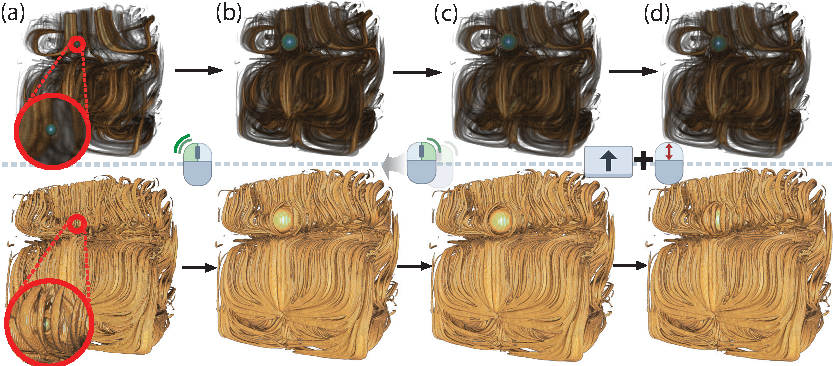
\includegraphics [width=\textwidth]{images/stream_lens.pdf} 
\caption{ A spherical item and its surrounding area are inspected using to our lens with 2 different transfer functions. The first part is displayed with transparency in opposition to the part below. The opacity helps to see the shape of the surrounding whirlpool. (a-a') The streamline dataset displayed using our framework. A dense object is hidden inside a whirlpool. (b-b') The lens tool is applied to the partially hidden object (double-click). The area is magnified and the occluding part of the whirlpool located in front of the spherical item is pushed aside. (c-c') The directions of the rays inside the lens are modified to see the whole sphere through the lens (right click+ mouse drag toward the desired direction). (d-d') The occluding part of the whirlpool can be restored/pushed gradually while keeping the area magnified (Shift + scroll).  }
\label{f:stream_lens}
\end{figure*}

\begin{figure} 
\includegraphics [width=0.45\textwidth]{images/streamline_orientation.pdf} 
\caption{ This figure shows 2 visualizations of a streamlines dataset. (a) The transfer function used allows to spot a spherical dense item inside the volume thanks to transparency. (b) This spherical object become occluded when the opacity of the surrounding whirlpool is increased in order to analyze its shape and behavior. }
\label{f:streamLineSTDViz}
\end{figure}
After the selection of a target, the lens offers a smooth transition between the previous view and the new one using a  slow-in/slow-out technique~\cite{Dragicevic:2011:TDA:1978942.1979233}. With this animation, the increase of the gradual speed at the beginning of the animation helps the user to start tracking the moving obstacles, and the decreasing speed at the end allows the user to predict where these occluding items stop moving. This also gives some semantic to the moving shapes, allowing the human mind to interpret the motion as a magnification of a target, and to keep the focus on visual entities during this transition. 

